% Created 2021-04-03 sáb 00:34
% Intended LaTeX compiler: pdflatex
\documentclass[11pt]{article}
\usepackage[utf8]{inputenc}
\usepackage[T1]{fontenc}
\usepackage{graphicx}
\usepackage{grffile}
\usepackage{longtable}
\usepackage{wrapfig}
\usepackage{rotating}
\usepackage[normalem]{ulem}
\usepackage{amsmath}
\usepackage{textcomp}
\usepackage{amssymb}
\usepackage{capt-of}
\usepackage{hyperref}
\author{Claudio Vaucheret}
\date{\today}
\title{Interpretación Abstracta de Programas Logicos}
\hypersetup{
 pdfauthor={Claudio Vaucheret},
 pdftitle={Interpretación Abstracta de Programas Logicos},
 pdfkeywords={},
 pdfsubject={},
 pdfcreator={Emacs 26.1 (Org mode 9.4)}, 
 pdflang={English}}
\begin{document}

\maketitle
\tableofcontents


\section*{Introducción}
\label{sec:org2daf528}

\begin{itemize}
\item analisis / sintesis de programas (Ciencias de la Computación)

\item Probar que un programa \(P\) tiene tal propiedad (analisis de programas)

\item Alternativamente: Derivar propiedades que tiene el programa \(P\)

\item Dado Un programa \(P\), generar un programa \(P'\) que sea:

\begin{itemize}
\item en algún sentido equivalente a P

\item funcione mejor que \(P\) con respecto a algún criterio
\end{itemize}
(analisis / sintesis de programas)

\item Aproximación Estandard:
\begin{itemize}
\item identificar que ocurre algún invariante y
\item especializar el programa para el caso particular
\end{itemize}
\end{itemize}

\section*{Analisis de Programas}
\label{sec:org3040579}

\begin{itemize}
\item Frecuente en compiladores aunque raramente tratados en modo formal:
\begin{itemize}
\item "optimización de código"
\item "eliminación de codigo muerto"
\item "movimiento de código"
\item \ldots{}
\end{itemize}
\item Interpretación Abstracta provee un marco formal para desarrollar
herramientas de análisis de programas
\item Fase de Análisis + fase de sintesis ≡ Interpretación Abstracta +
Transformación de Programas
\end{itemize}


\section*{¿Qué es la Interpretación Abstracta?}
\label{sec:orge662b7a}

\begin{itemize}
\item Considere detectar que una rama no ocurre: 
\begin{verbatim}
int x,y,z; y:=read(file); x:= y * y;
if x >= 0 then z := 1 else z:= 0

\end{verbatim}
\begin{itemize}
\item Analisis Exhaustivo en el dominio estandard: no termina
\item Razonamiento humano de los programas - Usa abstracciones o
aproximaciones: signos, ordenes de magnitud, par/impar, \ldots{}
\item Idea Básica: usar representaciones \emph{aproximadas} (generalmente
finitas) de los objetos computacionales para hacer tratable el
problema del analisis del flujo del programa
\end{itemize}
\item Analisis Abstracto es la formalización de esta idea:
\begin{itemize}
\item define una semantica no estandard que puede aproximar el
\emph{significado} o \emph{funcionamiento} del programa en un modo finito
\item las expresiones son computadas en un dominio (abstracto)
aproximado en lugar del dominio concreto.
\end{itemize}
\end{itemize}

\section*{Ejemplo: La regla de los signos}
\label{sec:org5e371e7}

\begin{itemize}
\item Consideremos el dominio \(D = Z\) (enteros)
\item y el operador de multiplicación: \(* : Z^2 \to Z\)
\item Definimos un \textbf{dominio abstracto}: \(D_\alpha = \{[-],[+]\}\)
\item y la multiplicación abstracta \(*_\alpha : {D_\alpha}^2 \to D_\alpha\)
definido por: 
\begin{center}
\begin{tabular}{lll}
\(*_\alpha\) & \([-]\) & \([+]\)\\
\hline
\([-]\) & \([+]\) & \([-]\)\\
\([+]\) & \([-]\) & \([+]\)\\
\hline
\end{tabular}
\end{center}
\item Esto nos permite razonar, por ejemplo, que \(y=x^2=x*x\) nunca es
negativo
\end{itemize}

\subsection*{Algunas observaciones:}
\label{sec:org592f0e8}
\begin{itemize}
\item si tenemos \(z = x * y\) entonces:
si \(x,y \in Z\) son aproximados con \(x_\alpha, y_\alpha \in
    D_\alpha\) entonces \(z \in Z\) es aproximado con \(z_\alpha = x_\alpha * y_\alpha\)
\item Es importante formalizar esta noción de aproximación para poder
probar que un análisis es correcto
\item La computación aproximada es generalmente menos precisa pero mas rápida.
\end{itemize}





\section*{Ejemplo: La regla de los signos (cont.)}
\label{sec:orga40c067}

\begin{itemize}
\item De nuevo \(D = Z\) (enteros)
\item y el operador \(* : Z^2 \to Z\)
\item Definimos un \emph{mas refinado} \textbf{dominio abstracto}: \(D'_\alpha = \{[-],[0],[+]\}\)
\item y la multiplicación abstracta \(*_\alpha : {D'_\alpha}^2 \to D'_\alpha\)
definido por: 
\begin{center}
\begin{tabular}{llll}
\(*_\alpha\) & \([-]\) & \([0]\) & \([+]\)\\
\hline
\([-]\) & \([+]\) & \([0]\) & \([-]\)\\
\([0]\) & \([0]\) & \([0]\) & \([0]\)\\
\([+]\) & \([-]\) & \([0]\) & \([+]\)\\
\hline
\end{tabular}
\end{center}
\item Esto nos permite razonar, que \(z=y*(0*x)\) es cero
\end{itemize}
\subsection*{Algunas observaciones:}
\label{sec:org28fc0e5}
\begin{itemize}
\item Hay un grado de libertad en definir operadores abstractos y
dominios diferentes
\item El requerimiento mínimo es que sea \textbf{seguro} o \textbf{correcto}
\item Definiciones "seguras" diferentes llevan a clase de análisis diferentes
\end{itemize}



\section*{Ejemplo: La regla de los signos (cont.)}
\label{sec:org220eea4}

\begin{itemize}
\item De nuevo \(D = Z\) (enteros)
\item y el operador de \emph{suma} \(+ : Z^2 \to Z\)
\item No podemos usar: \(D'_\alpha = \{[-],[0],[+]\}\) porque no sabríamos
como representar el resultado de \([+] +_\alpha [-]\) (i.e. la suma
abstracta no sería cerrada)
\item Un nuevo elemento "\(\top\)" (supremum) que es la aproximación para todo entero
\item Nuevo \textbf{dominio abstracto}: \(D''_\alpha = \{[-],[0],[+],\top\}\)
\end{itemize}

\subsection*{suma abstracta}
\label{sec:org2d11930}
\begin{itemize}
\item \(+_\alpha : {D''_\alpha}^2 \to D''_\alpha\)
definido por: 
\begin{center}
\begin{tabular}{lllll}
\(+_\alpha\) & \([-]\) & \([0]\) & \([+]\) & \(\top\)\\
\hline
\([-]\) & \([-]\) & \([-]\) & \(\top\) & \(\top\)\\
\([0]\) & \([-]\) & \([0]\) & \([+]\) & \(\top\)\\
\([+]\) & \(\top\) & \([+]\) & \([+]\) & \(\top\)\\
\(\top\) & \(\top\) & \(\top\) & \(\top\) & \(\top\)\\
\hline
\end{tabular}
\end{center}
\item Esto nos permite ahora razonar que \(z=x^2 + y^2\) nunca es negativo
\end{itemize}


\section*{Observaciones Importantes}
\label{sec:orga60cb6b}

\begin{itemize}
\item Además de la imprecisión debido a la "tosquedad" o lo "básico" de
\(D_\alpha\), las versiones abstractas de las operaciones
(que dependen de  \(D_\alpha\)) pueden introducir mas imprecisión
\item Así, la elección del \emph{dominio abstracto} y la definición de las
\emph{operaciones abstractas} son cruciales.
\end{itemize}


\section*{Propiedades de la Interpretación Abstracta}
\label{sec:org1fe09b0}
\begin{itemize}
\item Requeridas:
\begin{itemize}
\item Exactitud - aproximaciones correctas: a causa de que las
propiedades mas "interesantes" son indecidibles el análisis
necesariamente tiene que ser aproximado. Queremos asegurarnos de
que el análisis es "conservador" y se equivoca en el "lado seguro"
\item Terminación - la compilación definitivamente debe terminar
\end{itemize}
\item Deseable - "en la práctica"
\begin{itemize}
\item Eficiencia: en la práctica, el tiempo de análisis finito no es
suficiente: finito y pequeño
\item Precisión - de la información recopilada: depende de la idoneidad
de el dominio abstracto y el nivel de detalle al que el
procedimiento de interpretación imita la semántica del lenguaje
\item Utilidad: determina qué información vale la pena recopilar
\end{itemize}
\end{itemize}

\section*{Aproximaciones Correctas}
\label{sec:orgc763099}
\begin{itemize}
\item Idea básica en aproximación: para alguna propiedad \(p\) queremos mostrar
      $$\forall x, x \in S \Rightarrow p(x)$$ 
Alternativa: construir un conjunto \(S_a \supseteq S\) y demostrar
     $$\forall x, x \in S_a \Rightarrow p(x)$$ 
entonces, \(S_a\) es una aproximación segura de \(S\)
\item Aproximación de funciones: para alguna propiedad \(p\) queremos mostrar 
$$\forall x, x \in S \Rightarrow p(F(x))$$
\item Una función
$$G: S \rightarrow S$$ es una aproximación segura de \(F\) si
$$\forall x, x \in S, p(G(x)) \Rightarrow p(F(x))$$
\end{itemize}

\section*{Aproximación del significado de un programa}
\label{sec:orgb355e45}

\begin{itemize}
\item El significado de un programa \(P\) es un mapeo \(F_P\) de entrada a
salida, cuyos valores de  entrada y salida \(\in\) a un dominio
"estándar" \(D\): $$F_P: D \rightarrow D$$
\item "Elevemos" este significado para asignar \emph{conjuntos} de entradas a
\emph{conjuntos} de salidas $$F^*_P: \wp(D) \rightarrow \wp(D)$$ donde \(\wp(S)\)
denota el conjunto potencia de S, y $$F_P^*(S) = \{F_P(x) \arrowvert x \in  S\}$$
\item Una función $$G: \wp(D) \rightarrow \wp(D)$$ es una aproximación segura de
\(F_P^*\) si  $$\forall S, S \in \wp(D), G(S) \supseteq F_P^*(S)$$
\item Las propiedades se pueden demostrar usando \(G\) en lugar de \(F_P^*\)
\end{itemize}

\section*{Aproximación del significado de un programa (cont.)}
\label{sec:org321dc84}

\begin{itemize}
\item Para alguna propiedad \(p\) queremos mostrar que para las
entradas - \(S, p(F_P^*(S))\)
\item mostramos que para las entradas \(S_a, p(G(S_a))\)
\item Dado que \(G(S_a) \supseteq F_P^*(S_a)\) para las entradas \(S_a, p(F_P^*(S_a))\)
(Nota: abuso de notación - \(F_P^*\) no funciona con valores abstractos \(S_a\))
\item Siempre que \(F_P^*\) sea monótono: $$S_a \supseteq S \Rightarrow F_P^*(S_a) \supseteq F_P^*(S)$$
\item Y como \(S_a \supseteq S\), entonces: para las entradas \(S, p(F_P^*(S))\)
\end{itemize}


\section*{Dominio abstracto y función de concretización}
\label{sec:orgae22660}

\begin{itemize}
\item El dominio \(\wp(D)\) se puede representar mediante un dominio
"abstracto" \(D_\alpha\) de representaciones finitas de (posiblemente) objetos infinitos en \(\wp(D)\)
\item La representación de \(\wp(D)\) por \(D_\alpha\) se expresa mediante una
función (monótona) llamada función de concretización: $$\gamma :
  D_\alpha → \wp(D)$$ tal que \(\gamma(\lambda) = d\) si \(d\) es el
elemento más grande (bajo \(\supseteq\)) de \(\wp(D)\) que \(\lambda\)
describe [\((\wp(D), \supseteq)\) es obviamente una retículo completo]
\end{itemize}

\subsection*{Ejemplo}
\label{sec:org09e5d10}
\begin{itemize}
\item En el ejemplo de los "signos", con \(D_\alpha =
  \{[-],[0],[+],\top \}\), \(\gamma\) viene dado por \[
  \begin{align}
     \gamma([-]) &= \{x \in Z \arrowvert x < 0  \} \\
     \gamma([0]) &= \{0\} \\
     \gamma([+]) &= \{x \in Z \arrowvert x > 0\} \\
     \gamma(\top) &= Z \\
     \end{align} \]
\item \(\gamma(?) = \emptyset \rightarrow\) definimos \(\bot \arrowvert \gamma(\bot) = \emptyset\)
\end{itemize}


\section*{Función de abstracción}
\label{sec:orgca2fb50}

También podemos definir (no estrictamente necesario) una función de
 abstracción (monótona) $$\alpha : \wp(D) \rightarrow D_\alpha$$
 \(\alpha(d) = \lambda\) si \(\lambda\) es el elemento "mínimo" de
 \(D_\alpha\) que describe \(d\) [bajo un orden adecuado definido en los
 elementos de \(D_\alpha\)] 

p.ej. en el ejemplo de los "signos", \[
  \begin{align}
       \alpha(\{1, 2, 3\}) &= [+] (no \top) \\
       \alpha(\{- 1, −2, −3\}) &= [-] (no \top) \\
       \alpha(\{0\}) &= [0] \\
       \alpha(\{- 1, 0, 1\}) &= \top \\
     \end{align} \]
  \begin{center}

\includegraphics[width=.9\linewidth]{alphagamma2.png}
\end{center}


\section*{Significado abstracto y seguridad}
\label{sec:org4be91d5}
\begin{itemize}
\item Ahora podemos definir una función de significado abstracto como
$$F_\alpha : D_\alpha \rightarrow D_\alpha$$ que es segura si
$$\forall \lambda, \lambda \in D_\alpha, \gamma(F_\alpha(\lambda))
  \supseteq F^*_P(\gamma(\lambda))$$
	   \begin{center}

\includegraphics[width=.9\linewidth]{absmean2.png}
\end{center}
\item Entonces podemos probar una propiedad de la salida de una clase
dada de entradas, probando que todos los
elementos de \(\gamma(F_\alpha(\lambda))\) tienen tal propiedad
\item P.ej. puede demostrarse, una propiedad como "si este programa toma
un número positivo producirá un número negativo como salida"
\end{itemize}



\section*{Demostrar propiedades en abstracto}
\label{sec:org92725b4}
\begin{itemize}
\item Generando \(F_\alpha\):
\begin{itemize}
\item \(F_P\) obtenido del programa y la semántica predefinida de
operadores \((x + z) ∗ 3\), \(F_P = (x + z) ∗ 3\)
\item Análisis automático: \(F_\alpha\) debería obtenerse del programa y
la semántica de operadores abstractos (propiedades compositivas)
\(\{odd, even, +_\alpha, ∗_\alpha\} \Rightarrow F_\alpha = (x +_\alpha z) ∗_\alpha odd\)
\end{itemize}
\item "Si este programa toma un número positivo, producirá un número
negativo como salida"
\end{itemize}
\begin{itemize}
\item \(P = (y := x ∗ −3)\), entrada \(x\), salida \(y\)
\item \(F_P = x ∗ −3\)
\item \(F_\alpha = x ∗_\alpha [-]\)
\item \(F_\alpha([+]) = [+] ∗_\alpha [-] = [-]\)
\end{itemize}

\section*{Semánticas Colectoras}
\label{sec:org7785a78}
\begin{itemize}
\item La semántica de "entrada-salida" es a menudo demasiado tosca para un
análisis útil: información sobre el "Estado" en los puntos de
programa generalmente requieren \(\to\) "semánticas extendidas"
\item Los puntos del programa se pueden alcanzar muchas veces, desde
diferentes puntos y en diferentes "Estados" \(\to\) "semanticas
colectoras" 
   $$\{x> 3\} y := x ∗ −3 \{y < −9 \} \mbox{ o } \{x < −3\} y := x ∗ −3 \{y > 9 \}$$ 
   $$\{x = [+]\} y := x ∗ −3 \{y = [-]\} \mbox{ o } \{x = [-]\} y := x ∗ −3 \{y = [+]\}$$
\item El análisis a menudo calcula una colección de estados abstractos
para un punto de programa.  $$\{x = \{[+], [-]\}\} y := x ∗ −3 \{y = \{[-], [+]\}\}$$
\item A menudo, es más eficiente "resumir" estados en uno que ofrezca la
mejor descripción \(\to\)  estructura de retículo en un dominio abstracto $$\{x = \sqcup \{[+], [-]\}\} y := x ∗ −3 \{y = \sqcup \{[-], [+]\}\}$$
\end{itemize}

\section*{Estructura de Retículo}
\label{sec:org08e7ba6}
\begin{itemize}
\item El ordenamiento en \(\wp(D), \subseteq\), induce un ordenamiento en
\(D_\alpha, \leq_\alpha\) ("se aproxima mejor") Por ejemplo, podemos
elegir \(\alpha(\{1, 2, 3\}) = [+] \mbox{ o } \alpha(\{1, 2, 3\}) =
  \top\), pero \(\gamma([+]) = \{x \in Z \arrowvert x > 0\} \mbox{ y }
  \gamma(\top) = Z\), y dado que \(\{x \in Z \arrowvert x > 0\}
  \subseteq Z\) tenemos  \([+] \leq_\alpha \top\), es decir, \([+]\) se
aproxima mejor que \(\top\), es mas preciso.
\item Generalmente se requiere que \((D_\alpha, \leq_\alpha)\) sea una retículo completo
\item Por lo tanto, para todo \(S \subseteq D_\alpha\) existe un único
mínimo límite superior \(\sqcup S \in D_\alpha\), es decir, tal que
\begin{itemize}
\item \(\forall \lambda_S \in S, \lambda_S \leq_\alpha \sqcup S\)
\item \((\forall \lambda_S \in S, \lambda_S \leq_\alpha \lambda) \Rightarrow \sqcup S \leq_\alpha \lambda\)
\end{itemize}
\item Intuición: dado un conjunto de aproximaciones del "estado actual" en
un punto dado en un programa, para asegurarse de que sea la mejor
descripción "general" para el punto:
\begin{itemize}
\item \(\sqcup S\) se aproxima a \emph{todos} los elementos de \(S\)
\item \(\sqcup S\) es la mejor aproximación en \(D_\alpha\)
\end{itemize}
\end{itemize}

\section*{Ejemplo: aritmética entera de signos}
\label{sec:org2b2053f}
\begin{itemize}
\item Consideramos \(D_\alpha = \{[-], [0], [+],\top\}\)
\end{itemize}
\begin{itemize}
\item Agregamos \(\bot\) (infimum) para que \(\alpha(\emptyset)\) exista y
para tener una retículo completo: \(D_\alpha = \{\bot, [-], [0],
    [+], \top\}\)
\item (Intuición: representa un punto del programa que nunca será alcanzado)
\item La función de concretización debe ampliarse con $$\gamma(\bot) =
    \emptyset$$
\item El reticulo es:
\begin{center}

\includegraphics[width=.9\linewidth]{reticulo2.png}
\end{center}
\item \(\sqcup\{[+],[-]\} = \sqcup\{[-],[+]\} = \top\)
\end{itemize}

\section*{Ejemplo: aritmética entera de signos (cont.)}
\label{sec:org1ffe628}
\begin{itemize}
\item Para hacer \(t\) mas significativo, consideramos \(D_\alpha =
  \{\bot,[-],[0^-],[0],[0^+],[+],\top\}\)
\end{itemize}
\begin{center}
\begin{tabular}{lllllll}
\(\gamma(\bot)\) & \(=\) & \(\emptyset\) & \(\gamma(\top)\) & \(=\) & \(Z\) & \\
\(\gamma([-])\) & \(=\) & \(\{x \in Z \arrowvert x < 0 \}\) & \(\gamma([+])\) & \(=\) & \(\{x \in Z \arrowvert x > 0 \}\) & \(\gamma([0]) = \{0\}\)\\
\(\gamma([0^-])\) & \(=\) & \(\{x \in Z \arrowvert x \leq 0 \}\) & \(\gamma([0^+])\) & \(=\) & \(\{x \in Z \arrowvert x \geq 0 \}\) & \\
\end{tabular}
\end{center}
\begin{itemize}
\item El reticulo es: \begin{center}
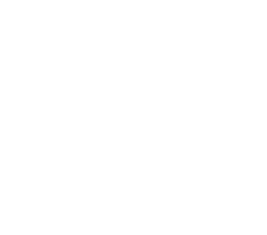
\includegraphics[width=.9\linewidth]{reticext2.png}
\end{center}
\item \(\sqcup\{[-],[0]\} = [0^-]\) representa con precisión un punto del programa donde una variable puede ser negativa o cero
\end{itemize}


\section*{El enfoque de la inserción de Galois}
\label{sec:orgb92d3d8}
\begin{itemize}
\item A continuación, nos referiremos a \(\wp(D)\) simplemente como \(D\)
\item Las semánticas (colectoras) de los programas a menudo son dadas por
\(lfp(F)\) (el mínimo \(S\) tal que \(S = F(S)\), Siendo \(F\) la función
semántica dependiente del programa en \(D\))
\item Por lo tanto, necesitamos relacionar este punto fijo con (el de) la
función semántica aproximada \(F_\alpha\) (que se aproxima a \(F\) y
opera sobre los elementos de un dominio abstracto \(D_\alpha\))
\item Suponga: \(D\) y \(D_\alpha\) son retículos completos; \(\gamma :
  D_\alpha \rightarrow D\) y \(\alpha : D \rightarrow D_\alpha\) son
funciones monotónicas. La estructura \((D_\alpha, \gamma, D, \alpha)\)
se denomina \emph{inserción de Galois} si:
\begin{itemize}
\item \(\forall \lambda \in D_\alpha . \lambda = \alpha(\gamma(\lambda))\)
\item \(\forall d \in D . d \subseteq \gamma(\alpha(d))\)
\end{itemize}
\end{itemize}
\subsection*{La \emph{Aproximación segura}}
\label{sec:org64df985}
\begin{itemize}
\item definida ahora en términos de una
inserción de Galois: Sea una inserción de Galois \((D_\alpha,
  \gamma,D, \alpha), \lambda \in D_\alpha\) aproxima en forma segura a
\(d \in D\)  ssi \(d \subseteq \gamma(\lambda)\)
\item Teorema fundamental [Cousot]: Dada una inserción de Galois
\((D_\alpha, \gamma, D, \alpha)\) y dos  funciones (monótonas) \(F: D
  \rightarrow D\) y \(F_\alpha: D_\alpha \rightarrow D_\alpha\) entonces
si \(F_\alpha\) es una aproximación de \(F\), \(lfp(F_\alpha)\) es una
aproximación de \(lfp(F)\)
\end{itemize}


\section*{Terminación: condiciones en \(F_\alpha\) y \(D_\alpha\)}
\label{sec:org7de3f15}
\begin{itemize}
\item La pregunta es si \(lfp(F_\alpha)\) es finitamente computable
\item El operador abstracto \(F_\alpha\) opera sobre los elementos de un
dominio abstracto \(D_\alpha\), que hemos requerido que sea un
retículo completo, y \(F_\alpha\) es monótona, por lo tanto
$$lfp(F_\alpha) = F_\alpha \uparrow n$$ para algún \(n\) que nos
gustaría sea finito (es decir, nos gustaría que la secuencia de Kleene fuera finita)
\item Recordando las características de los puntos fijos en retículos, la
secuencia de Kleene será finito en casos que incluyen:
\begin{itemize}
\item \(D_\alpha\) es finito
\item \(D_\alpha\) es cadena ascendente finita
\end{itemize}
\end{itemize}


\section*{Estructura de Retículos}
\label{sec:org80c815c}

\begin{center}
\begin{tabular}{ll}
finito & cadena finita ascendente\\
\begin{center}

\includegraphics[width=.9\linewidth]{finito2.png}
\end{center} & \begin{center}

\includegraphics[width=.9\linewidth]{chain2.png}
\end{center}\\
finito en profundidad & \\
\begin{center}
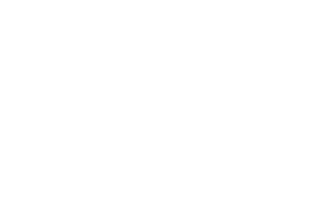
\includegraphics[width=.9\linewidth]{finitedepht2.png}
\end{center} & \\
\end{tabular}
\end{center}


\section*{Terminación: Discusión}
\label{sec:orgf2c011e}
\begin{itemize}
\item Demostrar la monotonicidad de \(F_\alpha\) puede ser más difícil que
mostrar que \(D_\alpha\) cumple con las condiciones de finitud
\item Puede haber un \(F_\alpha\) que termina incluso si no se cumplen las condiciones
\item Las condiciones también se relajan restringiendo la clase de
programas (por ejemplo, los programas no recursivos presentan pocas dificultades, aunque apenas son interesantes)
\item En algunos casos, una aproximación desde arriba (\(gfp(F_\alpha)\)) también puede ser interesante
\item Existen otras alternativas a la finitud: profundidad acotada
dinámica, etc. (Ver: widening y narrowing)
\end{itemize}

\section*{Análisis de programas lógicos}
\label{sec:org4fa0ef8}
\begin{itemize}
\item ¿Qué semántica?
\begin{itemize}
\item Semántica declarativa: relacionada a qué es una consecuencia del programa
\begin{itemize}
\item Semántica de la teoría de modelos mínimos
\item Semántica de punto fijo (basada en el operador \(T_P\))
(cf. estilo de base de datos, evaluación bottom-up )
\end{itemize}
\item Semántica operativa: cercana al comportamiento del programa
\begin{itemize}
\item Basado en resolución SLD (conjuntos éxitosos)
\item Denotacional
\item Puede cubrir posibilidades distintas a SLD: reactivo, paralelo, \ldots{}
\end{itemize}
\end{itemize}
\item Los análisis basados en semántica declarativa a menudo se denominan análisis \textbf{bottom up}
\item Los análisis basados en la semántica operativa (de arriba hacia
abajo) a menudo se denominan Análisis \textbf{top down}
\item Además, casos intermedios (generalmente logrados mediante la
transformación de programas)
\end{itemize}


\section*{Caso de Estudio: Semántica de punto fijo}
\label{sec:orgf473be6}
\begin{itemize}
\item Dado el lenguaje de primer orden \(L\) asociado con un programa \(P\)
dado, el universo de Herbrand (\(U\)) es el conjunto de todos los
términos básicos de \(L\).
\item La Base de Herbrand (\(B\)) es el conjunto de todos los átomos
instanciados (\emph{ground}) de \(L\).
\item Una \emph{interpretación de Herbrand} es un subconjunto de \(B\). \(I\) es el
conjunto de todas las interpretaciones de Herbrand (\(\wp(B)\))
\item Un \emph{modelo de Herbrand} es una interpretación de Herbrand que contiene
todos las consecuencias del programa.
\item El operador de consecuencia inmediata (\(T_P\)) es un mapeo \(T_P : I
  \rightarrow I\) definido por: $$T_P(M) = \{h \in B \vert \exists C
  \in ground(P), C = h \leftarrow b_1, \ldots, b_n \mbox{ y } b_1, \ldots,
  b_n \in M\}$$ (en particular, si (\(a \leftarrow\)) \(\in\) \(P\), entonces \(ground(a) \subseteq T_P(M)\), para cada \(M\)).
\item \(T_P\) es monótono, por lo que tiene un minimo punto fijo \(lfp(T_P)\)
que se puede obtener como \(T_P \uparrow \omega\) comenzando desde el
elemento inferior del retículo (la interpretación vacía, \(\emptyset\)).
\item (Teorema de caracterización) [Van Emden y Kowalski]: El menor modelo de Herbrand \(P\), \(H\) es \(lfp(T_P)\)
\end{itemize}

\section*{Semántica de punto fijo: Ejemplo}
\label{sec:org7398bf9}

\(P = \{ p(f(X)) \leftarrow p(X). \\
        p(a). q(a). q(b). \}\)

\begin{align}
U &= \{ a,b,f(a),f(b),f(f(a)),f(f(b)),\ldots \} \\

B &= \{ p(a),p(b),q(a),q(b),p(f(a)),p(f(b)),p(f(f(a))), \\ 
     p(f(f(b))), q(f(a))\ldots  \} \\

I &= \mbox{ todos los subconjuntos de } B \\

H &= \{ q(a), q(b), p(a), p(f(a)), p(f(f(a))), \ldots \} \\
\end{align}      

\begin{align}
T_P \uparrow 0 &= \{ p(a),q(a),q(b) \}\\

T_P \uparrow 1 &= \{ p(a),q(a),q(b),p(f(a)) \} \\

T_P \uparrow 2 &= \{ p(a),q(a),q(b),p(f(a)),p(f(f(a))) \} \\

\ldots \\

T_P \uparrow \omega &= H \\
\end{align}      


\section*{Interpretación abstracta "Bottom up"}
\label{sec:org7a14720}
\begin{itemize}
\item Encuentra una aproximación de \(H\) al aproximar \(lfp(T_P)\)
\item Aplicamos interpretación abstracta:
\begin{itemize}
\item Dominio: \(I^\alpha\), tal que elementos de \(I^\alpha\) son
aproximaciones de elementos de \(I = \wp(B)\).
\item Función de concretización: \(\gamma: I^\alpha \rightarrow I\)
\item Función de abstracción: \(\alpha: I \rightarrow I^\alpha\)
\item Operador Abstracto: versión abstracta del operador \(T_P\)
\(T^\alpha_P : I^\alpha \rightarrow I^\alpha\)
\end{itemize}
\end{itemize}
\subsection*{Interpretación abstracta "Bottom up" (cont.)}
\label{sec:orgfe02350}
\begin{itemize}
\item Aplicamos interpretación abstracta:
\begin{itemize}
\item Exactitud:
\begin{itemize}
\item \((I^\alpha, \gamma, I, \alpha)\) debe ser una inserción de
Galois, es decir, \(I^\alpha\) retículo completo y debería
aproximar a \(I: \forall M \in I, \gamma(\alpha(M)) \supseteq M\)
\item \(T^\alpha_P\) aproximación segura de \(T_P\), es decir, \(\forall d,
      d \in  I^\alpha, \gamma(T^\alpha_P(d)) \supseteq T_P(\gamma(d))\)
\end{itemize}
\item Terminación:
\begin{itemize}
\item \(T^\alpha_P\) es monótono.
\item \(I^\alpha\) (al menos) cadena ascendente finita.
\end{itemize}
\end{itemize}
\item Entonces, \(H^\alpha = lfp(T^\alpha_P) = T^\alpha_P \uparrow n\) se
obtendrá en un número finito de pasos \(n\) y \(H^\alpha\) se aproximará a \(H\).
\end{itemize}


\subsection*{Interpretación abstracta "Bottom up" (cont.)}
\label{sec:orgc8af07e}

\begin{center}

\includegraphics[width=.9\linewidth]{bottomup2.png}
\end{center}


\section*{Ejemplo: simple inferencia de "tipos"}
\label{sec:orgbe8f2d2}
\begin{itemize}
\item Problema de "inferencia de tipo" mínimal [Sondergaard]: Aproximación
de qué predicados están en \(H\)
\item \(pred(a):\) denota el símbolo de predicado de un átomo \(a\)
\item \(B^\alpha = S\) (conjunto de símbolos de predicado en un programa
\(P\)) Entonces \(I^\alpha = \wp(S)\), lo llamamos \(S^*\)
\item Función de concretización:
\begin{itemize}
\item \(\gamma: S^* \rightarrow I\)
\item \(\gamma(D) = \{a \in B | pred(a) \in D \}\)
\end{itemize}
\item Función de abstracción:
\begin{itemize}
\item \(\alpha: I \rightarrow S^*\)
\item \(\alpha(M) = \{p \in S | \exists a \in M, pred(a) = p \}\)
\end{itemize}
\item \((S^*, \gamma, I, \alpha)\) es una inserción de Galois.
\end{itemize}

\subsection*{Ejemplo: simple inferencia de "tipos" (cont.)}
\label{sec:org8bab637}
\begin{itemize}
\item Versión abstracta de \(T_P\) (después de alguna simplificación): $$T_P
  \alpha: S^* \rightarrow S^*$$
\end{itemize}

\(T^\alpha_P(D) = \{p \in S | \exists C \in P, 
                     C = h \rightarrow b_1, \ldots, b_n, \\
                     pred(h) \leftarrow pred(b_1), \ldots , pred(b_n)
                     \equiv p \leftarrow p_1,\ldots , p_n, \\
                     \mbox{ y } p_1,\ldots , p_n \in D\}\)
\begin{itemize}
\item \(S^*\) finito (número finito de símbolos de predicado en el programa)
y \(T^\alpha_P\) monótona \(\to\) El análisis terminará en un número
finito de pasos \(n\) y \(H^\alpha = T^\alpha_P \uparrow n\) se aproxima a \(H\).
\end{itemize}


\subsection*{Ejemplo: simple inferencia de "tipos" (cont.)}
\label{sec:org9a6e6fd}

\begin{itemize}
\item Ejemplo:
\end{itemize}

$$P = \{p(f(X)) \leftarrow p(X). 
    p(a). 
    r(X) ← t(X,Y). 
    q(a). 
    q(b). \}$$

$$P_\alpha = \{p \leftarrow p. 
    p. 
    r ← t. 
    q.\} $$

\begin{itemize}
\item \(S = \{p/1, q/1, r/1, t/2\}\)

\item Abstracción: \(\alpha(\{p(a), p(b), q(a)\}) = \{p/1, q/1\}\)

\item Concretización:
\end{itemize}
\begin{align}
\gamma(\{p/1, q/1\}) &= \{A \in B | pred(A) = p/1 \vee pred(A) = q/1\} \\
&= \{p(a), p(b), p(f(a)), p(f(b)),\ldots, q(a), q(b), q(f(a)),\ldots \} \\
\end{align}

\begin{itemize}
\item Análisis:
\end{itemize}
\(T^\alpha_P \uparrow 0 = T^\alpha_P(\emptyset) = {p / 1, q / 1}\) \\
\(T^\alpha_P \uparrow 1 = T^\alpha_P(\{p/1, q/1\}) = \{p/1, q/1\} = T^\alpha_P \uparrow 0 = H^\alpha\)


\section*{Análisis \textbf{bottom up} basado en \(T_P\): Discusión}
\label{sec:org11ef9ee}
\begin{itemize}
\item Ventajas:
\begin{itemize}
\item Simple y elegante. Basado en la semántica declarativa de punto fijo
\item General: resultados independientes de la consulta
\end{itemize}
\item Desventajas:
\begin{itemize}
\item Información solo sobre "salida del procedimiento". Normalmente se
necesita información en varios puntos del programa en la compilación, por ejemplo, "patrones de llamada"
\item La “variable lógica” no es observada (usa datos
instanciados). Información sobre estado de instanciación,
sustituciones, etc. a menudo necesarios en la compilación
\item No dirigido a consultas: analiza el programa completo, no la parte
(y los modos) que corresponden al uso "normal" (expresado a través
de una consulta)
\end{itemize}
\end{itemize}

\section*{Análisis \textbf{Top down} (resumido)}
\label{sec:org7d35ab6}
\begin{itemize}
\item Definir una semántica concreta extendida (recolectora), derivada de
la resolución SLD, haciendo observable la información relevante.
\item Dominio abstracto: generalmente "sustituciones abstractas".
\item Operaciones abstractas: unificación, composición, proyección, extensión, \ldots{}
\item Función semántica abstracta: toma una forma de consulta (abstracción
del objetivo inicial o conjunto de metas iniciales) y el programa y
devuelve descripciones abstractas de la sustituciones en puntos relevantes del programa.
\item Las variables complican las cosas:
\begin{itemize}
\item corrección (debido al aliasing),
\item terminación (fusión de información relacionada con aliasing)
\end{itemize}
\item Las variables lógicas son, de hecho, punteros (que se comportan
bien): 
X = tree(N,L,R),L = nill, Y = N, Y = 3, \ldots{}

\item esto hace que el análisis de programas lógicos sea muy interesante (y bastante relevante para otros paradigmas).
\end{itemize}

\section*{Arbol AND-OR abstracto}
\label{sec:orga37ef83}
\begin{itemize}
\item Exploración del árbol \texttt{?- p.   h:- p1, ... pn.}
\begin{center}

\includegraphics[width=.9\linewidth]{arbolandor2.png}
\end{center}
\item Operacons Basicas:
\begin{itemize}
\item Procedure entry: de \(\lambda_{call}\) obtiene \(\beta1_{entry}\)
\item Entry-to-exit (b): de \(\beta1_{entry}\) obtiene \(\beta1_{exit}\)
\item Clause entry: de \(\beta1_{entry}\) obtiene \(\lambda_1\)     (y clause exit)
\item Body traversal: de \(\lambda_1\) obtiene \(\lambda_{n+1}\)  (iterativamente aplicando (a))
\item Procedure exit: de (each or all of the) \(\beta{i}_{exit}\) obtiene \(\lambda_{success}\)
\end{itemize}
\end{itemize}

\section*{Optimización de Punto Fijo}
\label{sec:orgd23c189}
\begin{itemize}
\item Punto fijo es requerido solo en los predicados recursivos:
\end{itemize}
\begin{center}

\includegraphics[width=.9\linewidth]{arbolrec2.png}
\end{center}
\begin{itemize}
\item Recursivo simple (a)
\item Mutuamente Recursivos (b)
 "Usa la sustitución de exito actual e itera hasta que el punto fijo
es alcanzado"
\end{itemize}

\section*{Ciaopp}
\label{sec:org1aeecb3}
\begin{itemize}
\item Entrada 
\begin{itemize}
\item Programas Lógicos
\item aserciones y extensiones sintácticas (opcionalmente)
\end{itemize}
\item Salida
\begin{itemize}
\item Mensajes de Errores
\item Programa Transformado con:
\begin{itemize}
\item Resultados de analisis (como aserciones)
\item Resultados de chequeo estático de aserciones
\item Aserciones de chequeo en tiempo de ejecución
\item Optimizaciones (especialización, paralelización, etc).
\end{itemize}
\end{itemize}
\end{itemize}


\section*{Aserciones}
\label{sec:orgce855f4}
\begin{itemize}
\item estado de las aserciones
\begin{itemize}
\item \texttt{check}  (default) -- Es la semántica intentada, para ser
chequeada, es la especificación del programa, ingresada por el usuario.
\item \texttt{trust} -- semántica real, ingresada por el usuario y creída por
el compilador (es una guía).
\item \texttt{true} o \texttt{false} -- semántica real, salida del compilador.
\item \texttt{checked} -- validación: es un \texttt{check} que ha sido probado. (igual
a \texttt{true}).
\end{itemize}
\item ejemplo
\begin{verbatim}
:- trust pred is(X,Y) => (num(X),numexpr(Y)).

:- check pred p/2 : list(int) * var => list(int) * int.
:- modedef +X : nonvar(X).
:- check pred sortints(+L,-SL) :: list(int) * list(int) + sorted(SL)
			       # "@var{SL} has same elements as @var{L}.".
\end{verbatim}
\end{itemize}

\section*{Propiedades del estado de éxito}
\label{sec:orgbc58564}
\begin{itemize}
\item Propiedades del estado de \textbf{éxito}.  Son similiares en naturaleza a
las \emph{postcondiciones} usadas en verificación de programas
\begin{verbatim}
:- success Goal => Postcond.
\end{verbatim}
 debe ser interpretada como "para toda llamada de la forma \texttt{Goal} que
tiene éxito, al momento del éxito \texttt{Postcond} debería ser verdadero".

\item Restricción de las aserciones a un subconjunto de las llamadas
\begin{verbatim}
:- success Goal : Precond => Postcond.
\end{verbatim}
 debe ser interpretada como "para toda llamada de la forma \texttt{Goal}
para la cual \texttt{Predcond} ocurre, si la llamada 
 tiene éxito, al momento del éxito \texttt{Postcond} debería ser verdadero".
\end{itemize}

\section*{Propiedades en la llamada y computación}
\label{sec:orgcdb0b6b}
\begin{itemize}
\item Propiedades en el estado de llamada de un predicado que pueden
aparecer en tiempo de ejecución. 
\begin{verbatim}
:- calls Goal : Cond.
\end{verbatim}
  se debe interpretar "toda llamada de la forma \texttt{Goal} debería
satisfacer \texttt{Cond}".
\item Propiedades de la computación
\begin{verbatim}
:- comp Goal : Precond  + Comp_prop.
\end{verbatim}
  se debe interpretar "para toda llamada de la forma \texttt{Goal} para la
cual \texttt{Precond} ocurre, \texttt{Comp\_prop} debería ocurrir también para la
computación de \texttt{Goal}".
\end{itemize}

\section*{Composición de Aserciones}
\label{sec:org586da94}
Para facilitar la escritura una aserción compuesta de un predicado
puede ser usado como azúcar sintáctico para las aserciones básicas. La
aserción compuesta siguiente

\begin{verbatim}
:- pred Pred : Precond => Postcond + Comp_prop.
\end{verbatim}
corresponde a la siguiente aserción de éxito:

\begin{verbatim}
:- success Pred : Precond => Postcond.
\end{verbatim}
si la aserción \texttt{pred} tiene un campo \texttt{=>} (y un campo
\texttt{:}). También corresponde a una aserción de computación de la forma:

\begin{verbatim}
:- comp Pred : Precond + Comp_prop.
\end{verbatim}
si la aserción \texttt{pred} tiene los campos \texttt{+} y \texttt{:} 

\section*{Ejemplo de aserciones compuestas}
\label{sec:org1e41ad1}
\begin{itemize}
\item Consideremos el programa clasico quicksort \texttt{qsort} . Podemos usar la
\end{itemize}
siguiente aserción para requerir que la salida del procedimiento
\texttt{qsort} sea una lista.

\begin{verbatim}
:- success qsort(A,B) => list(B).
\end{verbatim}
\begin{itemize}
\item alternativamente podemos requerir que \texttt{qsort} es llamado con una
lista en su primer argumento y tiene exito, entonces el segundo
argumento también sera una lista.

\begin{verbatim}
:- success qsort(A,B) : list(A) => list(B).
\end{verbatim}
\end{itemize}

La diferencia reside en que se espera que \texttt{B} sea una lista en los casos en que \texttt{A} sea una lista. 

\section*{Ejemplo de aserciones compuestas (cont.)}
\label{sec:orgb0a9142}
\begin{itemize}
\item Además podemos requerir que en todas las llamadas al predicado
\texttt{qsort} el primer argumento debe ser una lista:

\begin{verbatim}
:- calls qsort(A,B) : list(A).
\end{verbatim}

\item El procedimiento \texttt{qsort} debe ordenar cualquier lista. Asi,
requeriremos que todas las llamadas con una lista en el primer
argumento y una variable en el segundo no fallen:

\begin{verbatim}
:- comp qsort(A,B) : (list(A) , var(B)) + does_not_fail.
\end{verbatim}
\end{itemize}

\section*{Ejemplo de aserciones compuestas (cont.)}
\label{sec:orged019e6}

En lugar de todas estas aserciones se puede usar la compuesta:

\begin{verbatim}
:- pred qsort(A,B) : (list(A) , var(B)) => list(B) + does_not_fail.
\end{verbatim}
que es equivalente a: 

\begin{verbatim}
:- calls qsort(A,B) : (list(A), var(B)).
:- success qsort(A,B) : (list(A), var(B)) => list(B).
:- comp qsort(A,B) : (list(A) , var(B)) + does_not_fail.
\end{verbatim}

\section*{Ejemplo de aserciones compuestas (cont.)}
\label{sec:org104df81}

si queremos llamar a \texttt{qsort} con algo diferente a una variable en el
segundo argumento se debe agregar:

\begin{verbatim}
:- pred qsort(A,B) : (list(A) , var(B)) => list(B) + does_not_fail.
:- pred qsort(A,B) : list(A) => list(B).
\end{verbatim}
que es equivalente a: 

\begin{verbatim}
:- calls qsort(A,B) : ((list(A), var(B)) ; list(A)).
:- success qsort(A,B) : ((list(A), var(B)) ; list(A)). => list(B).
:- comp qsort(A,B) : (list(A) , var(B)) + does_not_fail.
\end{verbatim}

\section*{Tipos Regulares}
\label{sec:org1f0485f}

Tipos Regulares son propiedades cuyas definiciones son  \emph{"programas
regulares"}. Ejemplos:

\begin{verbatim}
:- regtype tree(X) # "X is a tree.".

tree(nil).
tree(t(_,L,R)):- 
     tree(L),
     tree(R).

:- regtype intlist(X) # "X is a list of integers"

intlist([]).
intlist([X|R]) :- int(X), intlist(R).
\end{verbatim}

\section*{Lenguaje de aserciones}
\label{sec:org46babe0}
\begin{itemize}
\item ejemplo de \texttt{pred/1} 
\begin{verbatim}
:- pred length(L,N) : list * var => list * integer 
# "Computes the length of L.".
:- pred length(L,N) : var * integer => list * integer  
# "Outputs L of length N.".
:- pred length(L,N) : list * integer => list * integer
# "Checks that L is of length N.".
\end{verbatim}
\item ejemplo de \texttt{pred/2}
\begin{verbatim}
:- check pred length(L,N) : list * var => list * integer.
\end{verbatim}

\item ejemplo de \texttt{comp/1}
\begin{verbatim}
:- comp append(Xs,Ys,Zs) : var * var * var + not_fail.
\end{verbatim}

\item \texttt{test} es similar a \texttt{success} pero especifica un caso de test como
parte de la especificación del predicado
\begin{verbatim}
:- test length(L,N) : ( L = [1,2,5,2] ) => ( N = 4 ).
\end{verbatim}
\end{itemize}

\section*{Lenguaje de aserciones (cont.)}
\label{sec:org0360769}

\begin{itemize}
\item definición de nuevos modos

\begin{verbatim}
:- modedef +A : nonvar(A) # "A is bound upon predicate entry.".

:- pred p(+A,B) : integer(A) =>  ground(B).
\end{verbatim}
es equivalente a:
\begin{verbatim}
:- pred p(A,B) : (nonvar(A),integer(A)) =>  ground(B)
			 # "A is bound upon predicate entry.".
\end{verbatim}

\item documentación 

\begin{verbatim}
:- doc(Pred,Comment). 

:- doc(p(A,B),"A is bound upon predicate entry.").
\end{verbatim}
\end{itemize}


\section*{Ciaopp}
\label{sec:org41e7bcc}

\begin{center}
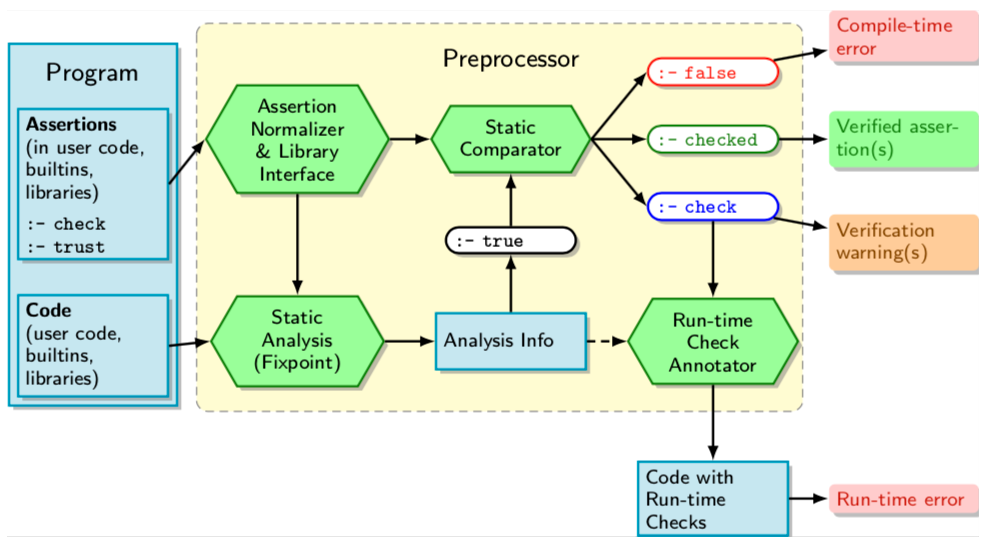
\includegraphics[width=.9\linewidth]{arquitectura.png}
\end{center}









\section*{Analisis}
\label{sec:orgb70d27d}
\begin{itemize}
\item Entrada
\begin{verbatim}
:- module(app, [app/3], [assertions]).

:- entry app(A,B,C) : (list(A), list(B)).

app([],Y,Y).
app([X|Xs], Ys, [X|Zs]) :- app(Xs,Ys,Zs).
\end{verbatim}

\item Salida 
\begin{verbatim}
:- true pred app(A,B,C) : ( list(A), list(B), term(C) )
			    => ( list(A), list(B), list(C) ).

:- true pred app(A,B,C) 
   : mshare([[A],[A,B],[A,B,C],[A,C],[B],[B,C],[C]])
   => mshare([[A,B,C],[A,C],[B,C]]).

\end{verbatim}
\end{itemize}

\subsection*{Analisis}
\label{sec:org0570065}
\begin{itemize}
\item Entrada
\begin{verbatim}
:- module(qsort, [qsort/2], [assertions]).

:- entry qsort(A,B) : (list(num, A), var(B)).

qsort([X|L],R) :-
    partition(L,X,L1,L2),
    qsort(L2,R2), qsort(L1,R1),
    append(R2,[X|R1],R).
qsort([],[]).

partition([],_B,[],[]).
partition([E|R],C,[E|Left1],Right):-
    E < C, !, partition(R,C,Left1,Right).
partition([E|R],C,Left,[E|Right1]):-
    E >= C, partition(R,C,Left,Right1).

append([],X,X).
append([H|X],Y,[H|Z]):- append(X,Y,Z).
\end{verbatim}
\end{itemize}

\subsection*{Analisis}
\label{sec:org11ee096}
\begin{itemize}
\item dominio shfr sin el \textasciitilde{}:- entry \ldots{} \textasciitilde{} 
\begin{verbatim}
:- true pred qsort(_A,R)
   : mshare([[_A],[_A,R],[R]])
   => mshare([[_A,R]]).

:- true pred partition(_A,_B,Left,Right)
   : ( mshare([[_A],[_A,_B],[_B],[Left],[Right]]), var(Left), var(Right) )
   => ( mshare([[_B]]), ground([_A,Left,Right]) ).

:- true pred append(_A,X,_B)
   : ( mshare([[X],[X,_B],[_B]]), ground([_A]) )
   => ( mshare([[X,_B]]), ground([_A]) ).
\end{verbatim}
\end{itemize}

\subsection*{Analisis}
\label{sec:orgd4d1a4d}
\begin{itemize}
\item dominio shfr con el \texttt{:- entry qsort(A,B) : (list(num, A), var(B)).} 
\begin{verbatim}
:- true pred qsort(A,B)
   : ( mshare([[B]]), var(B), ground([A]) )
   => ground([A,B]).

:- true pred partition(_A,_B,Left,Right)
   : ( mshare([[Left],[Right]]), var(Left), var(Right), ground([_A,_B]) )
   => ground([_A,_B,Left,Right]).

:- true pred append(_A,X,_B)
   : ( mshare([[_B]]), var(_B), ground([_A,X]) )
   => ground([_A,X,_B]).
\end{verbatim}
\end{itemize}

\subsection*{Analisis}
\label{sec:org69f0cbe}
\begin{itemize}
\item dominio eterms sin  \texttt{:- entry qsort(A,B) : (list(num, A), var(B)).} 
\begin{verbatim}
:- true pred qsort(_A,R)
   : ( term(_A), term(R) )
   => ( list(_A), list(R) ).

:- true pred partition(_A,_B,Left,Right)
   : ( term(_A), term(_B), term(Left), term(Right) )
   => ( list(arithexpression,_A), term(_B), 
	list(arithexpression,Left), list(arithexpression,Right) ).

:- true pred append(_A,X,_B)
   : ( list(_A), non_empty_list(X), term(_B) )
   => ( list(_A), non_empty_list(X), non_empty_list(_B) ).
\end{verbatim}
\end{itemize}

\subsection*{Analisis}
\label{sec:org9f4fbe1}
\begin{itemize}
\item dominio eterms con  \texttt{:- entry qsort(A,B) : (list(num, A), var(B)).} 
\begin{verbatim}
:- true pred qsort(A,B)
  : ( list(num,A), term(B) )
  => ( list(num,A), list(num,B) ).

:- true pred partition(_A,_B,Left,Right)
  : ( list(num,_A), num(_B), term(Left), term(Right) )
 => ( list(num,_A), num(_B), list(num,Left), list(num,Right) ).

:- true pred append(_A,X,_B)
 : ( list(num,_A), list1(num,X), term(_B) )
=> ( list(num,_A), list1(num,X), list1(num,_B) ).
\end{verbatim}
\end{itemize}

\section*{Debugging}
\label{sec:orgabe0345}
\begin{itemize}
\item Entrada
\begin{verbatim}
:- module(qsort, [qsort/2], [assertions]).

:- entry qsort(A,B) : (list(num, A), var(B)).

qsort([X|L],R) :-
    partition(L,X,L1,L2),
    qsort(L2,R2), qsort(L1,R1), 
    append(R2,[x|R1],R).    % <-- 'x' should be X (variable)
qsort([],[]).

partition([],_B,[],[]).
partition([E|R],C,[E|Left1],Right):- 
    E < C, !, partition(R,C,Left1,Right).
partition([E|R],C,Left,[E|Right1]):-
    E >= C,   partition(R,C,Left,Right1).

append([],X,X).
append([H|X],Y,[H|Z]):- append(X,Y,Z).

\end{verbatim}
\end{itemize}

\subsection*{Debugging}
\label{sec:orge7b379f}
\begin{itemize}
\item Salida
\begin{verbatim}
:- true pred qsort(A,B)
   : ( list(num,A), term(B) )
   => ( list(num,A), list(^(x),B) ).

\end{verbatim}
\end{itemize}

\subsection*{Debugging}
\label{sec:org76066a1}
\begin{itemize}
\item Entrada
\begin{verbatim}
:- module(_, [qsort/2], [assertions]).

:- entry qsort(A,B) : (list(num, A), var(B)).

qsort([X|L],R) :-
    partition(L,L1,X,L2),  % <-- swapped second and third arguments
    qsort(L2,R2), qsort(L1,R1),
    append(R2,[X|R1],R).
qsort([],[]).

partition([],_B,[],[]).
partition([e|R],C,[E|Left1],Right):-  % <-- 'e' should be E (variable)
    E < C, !, partition(R,C,Left1,Right).
partition([E|R],C,Left,[E|Right1]):-
    E >= C, partition(R,C,Left,Right1).

append([],X,X).
append([H|X],Y,[H|Z]):- append(X,Y,Z).
\end{verbatim}
\end{itemize}


\subsection*{Debugging}
\label{sec:org71c04f2}
\begin{itemize}
\item Salida
\begin{verbatim}
{In /home/claudio/tmp/orgfiles/data/ciaopp/clase2/hacerslides/debugging/qsort2.pl
WARNING (preproc_errors): (lns 4-8) goal qsort2:partition(L,L1,X,L2) at literal 1 does not succeed!
}
{ERROR (ctchecks_messages): error printing:message_clause_incompatible(qsort2:partition/4/2,eterms
 ,qsort2:partition([e|C],A,[D|E],B),[A,B,C,D,E],[C,Right,R,E,Left1])
}
{In /home/claudio/tmp/orgfiles/data/ciaopp/clase2/hacerslides/debugging/qsort2.pl
WARNING (preproc_errors): (lns 14-15) goal arithmetic:>=(E,C) at
literal 1 does not succeed!
\end{verbatim}
\end{itemize}


\subsection*{Debugging}
\label{sec:org4b98981}
\begin{itemize}
\item Chequear Aserciones
\begin{verbatim}
:- module(qsort3, [qsort/2], [assertions,regtypes,nativeprops]).

:- entry qsort(A,B) : (list(num, A), var(B)).

:- calls qsort(A,B) : list(num, A).                        % A1
:- success qsort(A,B)  => (ground(B), sorted_num_list(B)). % A2
:- calls partition(A,B,C,D) : (ground(A), ground(B)).      % A3
:- success partition(A,B,C,D) => (list(num, C),ground(D)). % A4
:- calls append(A,B,C) : (list(num,A),list(num,B)).        % A5

:- prop sorted_num_list/1.
sorted_num_list([]).
sorted_num_list([X]):- number(X).
sorted_num_list([X,Y|Z]):- 
    number(X), number(Y), X=<Y, sorted_num_list([Y|Z]).

qsort([X|L],R) :-
    partition(L,X,L1,L2),
    qsort(L2,R2), qsort(L1,R1),
    append(R2,[x|R1],R).
qsort([],[]).

partition([],_B,[],[]).
partition([E|R],C,[E|Left1],Right):-
    E < C, !, partition(R,C,Left1,Right).
partition([E|R],C,Left,[E|Right1]):-
    E >= C, partition(R,C,Left,Right1).

append([],X,X).
append([H|X],Y,[H|Z]):- append(X,Y,Z).
\end{verbatim}
\end{itemize}

\section*{Optimización}
\label{sec:orgf9bc468}
\begin{itemize}
\item Entrada
\begin{verbatim}
:- module(_, [dup_first/2], []).

dup_first([X|Xs], Zs) :-
    app([X], [X|Xs], Zs).

app([],Y,Y).
app([X|Xs], Ys, [X|Zs]) :-
    app(Xs,Ys,Zs).
\end{verbatim}

\item Salida 
\begin{verbatim}
:- module(_1,[dup_first/2],[assertions]).

dup_first([A|B],[A,A|B]).

\end{verbatim}
\end{itemize}

\subsection*{Optimización}
\label{sec:org5639fc4}
\begin{itemize}
\item Entrada
\begin{verbatim}
:- module(append,[appe/3],[assertions] ) .


:- entry appe(A,B,C). 

appe(A,B,C) :- append([1,2,3|A],B,C).

append([],X,X).
append([H|X],Y, [H|Z]):- append(X,Y,Z) .
\end{verbatim}

\item Salida 
\begin{verbatim}
:- module(_1,[appe/3],[assertions]).

:- entry appe(A,B,C).

appe([],A,[1,2,3|A]).
appe([B|C],A,[1,2,3,B|D]) :-
    append_1(C,A,D).

append_1([],A,A).
append_1([B|C],A,[B|D]) :-
    append_1(C,A,D).
\end{verbatim}
\end{itemize}

\subsection*{Optimización}
\label{sec:org770212b}
\begin{itemize}
\item Entrada
\begin{verbatim}
:- module(exponential_ac, [ent/2], [assertions]) .


:- entry ent(Base,_) : int(Base).

ent(Base,Res) :- exp(Base,3,Res).

exp(Base,Exp,Res):-
     exp_ac(Exp,Base,1,Res).

exp_ac(0,_,Res,Res).

exp_ac(Exp,Base,Tmp,Res) :-
    Exp > 0,
    Expl is Exp - 1,
    NTmp is Tmp * Base,
    exp_ac(Expl,Base,NTmp,Res).
\end{verbatim}
\end{itemize}
\subsection*{Optimizacion}
\label{sec:org2b6072a}
\begin{itemize}
\item Salida 
\begin{verbatim}
:- module(_1,[ent/2],[assertions]).

:- entry ent(Base,_A)
   : int(Base).

ent(A,B) :-
    C is A,
    D is C*A,
    E is D*A,
    exp_ac_1(A,E,B).

exp_ac_1(_1,A,A).

\end{verbatim}
\end{itemize}

\section*{Certificación}
\label{sec:org0a91cfd}
\begin{itemize}
\item Entrada
\begin{verbatim}
:- module(multiply,_,[assertions]).

:- entry mmultiply(X,Y,Z): (var(Z),list(X,list(num)),list(Y,list(num))).
:- entry mmultiply(X,Y,Z) : (var(Z),ground(X),ground(Y)). 


mmultiply([],_,[]).
mmultiply([VO|Rest],V1,[Result|Others]):-
    mmultiply(Rest,V1,Others),
    multiply(V1,VO,Result).

multiply([],_,[]).
multiply([VO|Rest],VI,[Result|Others]):-
    multiply(Rest,VI,Others),
    vmul(VO,VI,Result).

vmul([],[],0).
vmul([H1|T1],[H2|T2],Result):-
    vmul(T1,T2,Newresult),
    Product is H1*H2,
    Result is Product+Newresult.
\end{verbatim}
\end{itemize}

\subsection*{Certificación}
\label{sec:org0c9be03}
\begin{itemize}
\item Certificado
\begin{verbatim}
:- true pred A is B+C : (mshare([[A]]),var(A),ground([B,C]))
			  => (ground([A,B,C])).
:- true pred A is B*C : (mshare([[A]]),var(A),ground([B,C]))
			 => (ground([A,B,C])).

:- true pred A is B+C : (term(A),num(B),num(C))
			 => (num(A),num(B),num(C)).

:- true pred A is B*C : (term(A),num(B),num(C))
			 => (num(A),num(B),num(C)).
\end{verbatim}
\end{itemize}
\end{document}